\documentclass[resume]{subfiles}

\begin{document}
\section{Contrôlabilité}

Si l'ensemble des états que l'on peut atteindre en partant de zéro est l'espace d'états entier, alors le système est dit complètement contrôlable. (On peut aller partout)
\subsection{Matrice de contrôlabilité}
$$P_c=\begin{bmatrix}
\\
B & AB & A^2B & \cdots & A^{n-1}B\\
\\
\end{bmatrix}$$
$$\boxed{\det(P_c)\neq 0\longrightarrow\text{ Contrôlable}}$$





\subsection{Définition}

Le système $\dot{x}(t) = Ax(t)+Bu(t)$ est complètement contrôlable si pour $x(0)=0$ et pour tout état $x^*$ , il existe un temps fini $t^*$ et une entrée continue par morceaux $u(t)$ dans $[0,t^*]$ telle que $x(t^*)=x^*$ 

\subsection{Théorème}

Un système à temps continu (discret) est complètement contrôlable si, est seulement si, la matrice de contrôlabilité:
$M = [B, AB, A^2B,..., A^{n-1}B]$ est de rang n  (rang plein)

\subsection{Forme canonique contrôlabilité}

Une équation différentielle d'ordre n peut être remappée en un système de n équations du premier ordre

$\frac{d^ny}{dt^n} + a_1\frac{d^{n-1}y}{dt^{n-1}}+...+ a_ny=u$ 

On pose y=x1
\begin{align*}
\dot{x}_1 = x_2\\
\dot{x}_2 = x_3\\
\vdots\\
\dot{x}_{n-1} = x_n\\
\dot{x}_n = -a_1x_n -...- a_nx_1+u
\end{align*}

On a donc 
$$
A=\begin{bmatrix}
0 & 1 & 0 & \cdots & 0 \\
0 & 0 & 1 & \cdots & 0 \\
\vdots & \vdots & \vdots& \ddots & \vdots\\
0 & 0 & 0 & \cdots & 1 \\
-a_n & -a_{n-1}& -a_{n-2} &\cdots& -a_{1}
\end{bmatrix}$$

$$b=\begin{bmatrix}
0 \\
0 \\
\vdots\\
0 \\
1 \\
\end{bmatrix},
c=\begin{bmatrix}
1&0&\cdots&0 &0
\end{bmatrix}
$$
Le système (A,b,c) a des propriétés intéressantes, La dernière ligne est composée des coefficients du polynôme caractéristique

$\Delta_A(\lambda) = det (\lambda I - A) = \lambda^n + a_1\lambda^{n-1} +...+ a_n  $ 

Tout système complètement contrôlable est équivalent à un système sous forme canonique de contrôlabilité

\subsection{Transformation}

Il est possible de mettre tout système complètement contrôlable sous sa forme canonique par une simple transformation $x=Mz$ avec $M=[b|Ab|...|A^{n-1}b]$ 

On obtient $\bar{A}= M^{-1}AM$ qui est la forme canonique compagnon de contrôlabilité

\subsection{Rétroaction}

\subsubsection{Contrôle en boucle ouverte}
\begin{itemize}
\item la fonction d'entrée est déterminée par un process
  externe
\item exemple: un feu de circulation à cycle fixe
\end{itemize}

\subsubsection{Contrôle en boucle fermée}
\begin{itemize}
\item la commande est déterminée par le comportement du
  système
\item exemple: un thermostat
\item La boucle fermée est plus facile à réaliser
\item La boucle fermée requiert du temps de calcul  
\end{itemize}

\subsection{Retour d'état}

\begin{figure}[H]
    \centering
    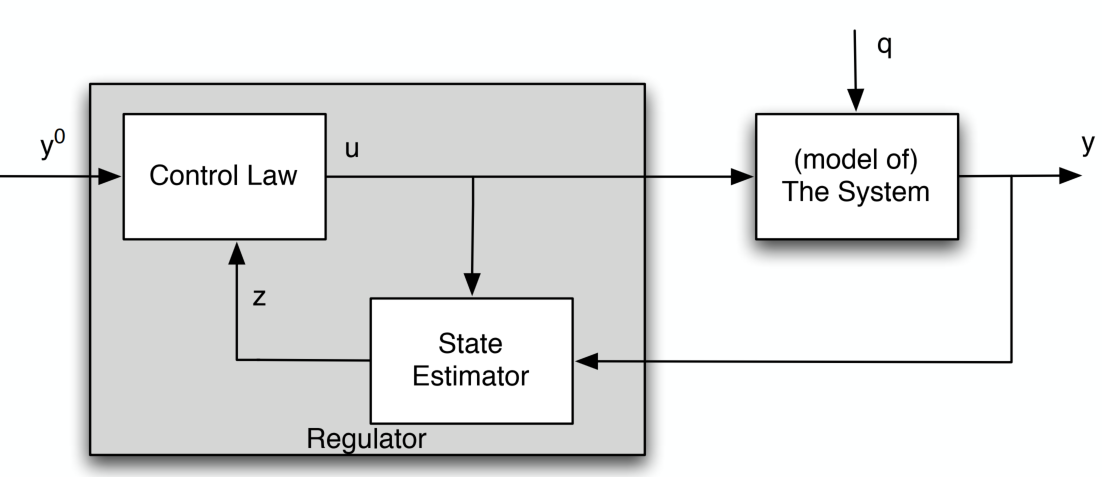
\includegraphics[width=1\columnwidth]{Figures/CtrlStab_2.png}
\end{figure}
$$u(t)=Kz(t)$$
La dynamique de la boucle ouverte est $A-BK$ (ou $A+BK$, c'est égal car on va déterminer les valeurs de $K$).

\subsubsection{Théorème}

Soit $(A, B)$ un système complètement contrôlable. Alors, pour tout choix d'un polynôme $p (\lambda)$ d'ordre n $p (\lambda) = \lambda^n + a_{n-1}\lambda^{n-1} +...+ a_0$,
il existe une matrice réelle $K$ telle que le polynôme caractéristique de est $A + BK$ est $p (\lambda)$ 

\end{document}